% answers.tex —— 2024 年·新高考Ⅰ卷 · 参考答案与详细解析片段
% 由 tools/generate_projects.py 依来源总账自 2024/2024_数学真题_试题.md + 2024/2024_数学真题_解析正文.md + 2024/2024_数学真题_答案要点.md 生成，勿手改（改源 MD 后重跑）


\begin{gknotice}
\textbf{解析归属}：本文档全部解析由本库编写者根据试题独立推导，\textbf{非官方标准答案}。推导过程完整给出以便核验；若与官方发布版本不一致，以官方为准。

\textbf{卷种提示}：2024 年是题型分水岭（19 题制），结构与 2025、2026 一致，是最贴近 2027 高考的对标真题之一。
\end{gknotice}

\par\medskip

\gkpart{一、单选题（每小题 5 分，共 40 分）}

\begin{answer}
\gksolhead{1}{}

\textbf{题目}：

已知集合 $A=\left\{x\mid -5<x^{3}<5\right\}$，$B=\{-3,-1,0,2,3\}$，则 $A\cap B=$（　　）

\begin{gkopts}(4)
\task A．$\{-1,0\}$
\task B．$\{2,3\}$
\task C．$\{-3,-1,0\}$
\task D．$\{-1,0,2\}$
\end{gkopts}

\textbf{解析}

\textbf{关键}：$y=x^{3}$ 在 $\mathbf R$ 上\textbf{单调递增}（且值域为 $\mathbf R$），因此对不等式两边同时开立方，不等号方向不变、也不需分类讨论：
\[-5<x^{3}<5\ \Longleftrightarrow\ -\sqrt[3]5<x<\sqrt[3]5\]

估算 $\sqrt[3]5$：因 $1.7^{3}=4.913<5<5.832=1.8^{3}$，故 $1.7<\sqrt[3]5<1.8$。

于是 $A\approx(-1.71,\ 1.71)$。逐个检验 $B$ 中元素：

\begin{center}
\begin{tabular}{cccccc}
\toprule
元素 & $-3$ & $-1$ & $0$ & $2$ & $3$ \\
\midrule
$x^3$ & $-27$ & $-1$ & $0$ & $8$ & $27$ \\
是否满足 $-5<x^3<5$ &  &  &  &  &  \\
\bottomrule
\end{tabular}
\end{center}

\[A\cap B=\{-1,\ 0\}\]

\begin{gktip}
\textbf{更快的做法}：不必求 $\sqrt[3]5$，直接把 $B$ 的五个元素\textbf{立方后}与 $(-5,5)$ 比较即可（上表第二行），心算一步到位。
\end{gktip}

\gkanswer{答案：A}

\par\medskip

\end{answer}
\begin{answer}
\gksolhead{2}{}

\textbf{题目}：

若 $\dfrac{z}{z-1}=1+\mathrm{i}$，则 $z=$（　　）

\begin{gkopts}(4)
\task A．$-1-\mathrm{i}$
\task B．$-1+\mathrm{i}$
\task C．$1-\mathrm{i}$
\task D．$1+\mathrm{i}$
\end{gkopts}

\textbf{解析}

交叉相乘去分母（注意 $z\ne1$）：
\[z=(1+\mathrm i)(z-1)=(1+\mathrm i)z-(1+\mathrm i)\]

移项，把含 $z$ 的项归并：
\[z-(1+\mathrm i)z=-(1+\mathrm i)\ \Longrightarrow\ \left[1-(1+\mathrm i)\right]z=-(1+\mathrm i)\ \Longrightarrow\ -\mathrm i\,z=-(1+\mathrm i)\]

\[z=\frac{1+\mathrm i}{\mathrm i}\]

分母实数化（分子分母同乘 $-\mathrm i$，或直接利用 $\dfrac1{\mathrm i}=-\mathrm i$）：
\[z=(1+\mathrm i)\cdot\frac1{\mathrm i}=(1+\mathrm i)(-\mathrm i)=-\mathrm i-\mathrm i^{2}=-\mathrm i+1=1-\mathrm i\]

\textbf{检验}（复数题必做）：
\[\frac{1-\mathrm i}{(1-\mathrm i)-1}=\frac{1-\mathrm i}{-\mathrm i}=\frac{(1-\mathrm i)\cdot\mathrm i}{-\mathrm i\cdot\mathrm i}=\frac{\mathrm i-\mathrm i^{2}}{1}=1+\mathrm i\quad\checkmark\]

\begin{gktip}
\textbf{常用小结论}：$\dfrac1{\mathrm i}=-\mathrm i$。记住它可以省掉一次乘共轭的运算。
\end{gktip}

\gkanswer{答案：C}

\par\medskip

\end{answer}
\begin{answer}
\gksolhead{3}{}

\textbf{题目}：

已知向量 $\boldsymbol a=(0,1)$，$\boldsymbol b=(2,x)$，若 $\boldsymbol b\perp(\boldsymbol b-4\boldsymbol a)$，则 $x=$（　　）

\begin{gkopts}(4)
\task A．$-2$
\task B．$-1$
\task C．$1$
\task D．$2$
\end{gkopts}

\textbf{解析}

先求出 $\boldsymbol b-4\boldsymbol a$：
\[\boldsymbol b-4\boldsymbol a=(2,x)-4(0,1)=(2,\ x-4)\]

由垂直 $\iff$ 数量积为零：
\[\boldsymbol b\cdot(\boldsymbol b-4\boldsymbol a)=2\times2+x(x-4)=0\]
\[4+x^{2}-4x=0\ \Longrightarrow\ x^{2}-4x+4=0\ \Longrightarrow\ (x-2)^{2}=0\]

\[x=2\]

\begin{gktip}
\textbf{注意}：$(x-2)^2=0$ 是\textbf{重根}，只有 $x=2$ 一个解。若下意识地写成「$x=2$ 或 $x=-2$」就会错选。
\end{gktip}

\gkanswer{答案：D}

\par\medskip

\end{answer}
\begin{answer}
\gksolhead{4}{}

\textbf{题目}：

已知 $\cos(\alpha+\beta)=m$，$\tan\alpha\tan\beta=2$，则 $\cos(\alpha-\beta)=$（　　）

\begin{gkopts}(4)
\task A．$-3m$
\task B．$-\dfrac m3$
\task C．$\dfrac m3$
\task D．$3m$
\end{gkopts}

\textbf{解析}

\textbf{核心技巧：整体设元。} 注意到两角和差的余弦公式只用到 $\cos\alpha\cos\beta$ 与 $\sin\alpha\sin\beta$ 这\textbf{两个整体}，而条件恰好也只涉及它们，因此不必去求 $\alpha$、$\beta$ 本身。

令
\[c=\cos\alpha\cos\beta,\qquad s=\sin\alpha\sin\beta\]

\textbf{由第二个条件}：
\[\tan\alpha\tan\beta=\frac{\sin\alpha\sin\beta}{\cos\alpha\cos\beta}=\frac sc=2\ \Longrightarrow\ s=2c\]

\textbf{由第一个条件}：
\[\cos(\alpha+\beta)=c-s=c-2c=-c=m\ \Longrightarrow\ c=-m\]

\textbf{代入所求}：
\[\cos(\alpha-\beta)=c+s=c+2c=3c=3(-m)=-3m\]

\begin{gktip}
\textbf{方法总结}：凡是「已知 $\cos(\alpha+\beta)$ 与 $\tan\alpha\tan\beta$（或类似组合）求 $\cos(\alpha-\beta)$」的题，一律设 $c$、$s$ 两个整体量，联立两个线性方程即可，\textbf{不要试图解出单个角}。
\end{gktip}

\gkanswer{答案：A}

\par\medskip

\end{answer}
\begin{answer}
\gksolhead{5}{}

\textbf{题目}：

已知圆柱和圆锥的底面半径相等，侧面积相等，且它们的高均为 $\sqrt3$，则圆锥的体积为（　　）

\begin{gkopts}(4)
\task A．$2\sqrt3\pi$
\task B．$3\sqrt3\pi$
\task C．$6\sqrt3\pi$
\task D．$9\sqrt3\pi$
\end{gkopts}

\textbf{解析}

设公共的底面半径为 $r$，高 $h=\sqrt3$。

\textbf{圆柱侧面积}（展开是矩形，长为底面周长、宽为高）：
\[S_{\text{\text{柱侧}}}=2\pi r\cdot h=2\sqrt3\,\pi r\]

\textbf{圆锥侧面积}（用\textbf{母线} $l$，不是高）：
\[l=\sqrt{r^{2}+h^{2}}=\sqrt{r^{2}+3},\qquad S_{\text{\text{锥侧}}}=\pi r l=\pi r\sqrt{r^{2}+3}\]

\textbf{由侧面积相等}（$r>0$，可约去 $\pi r$）：
\[2\sqrt3\,\pi r=\pi r\sqrt{r^{2}+3}\ \Longrightarrow\ 2\sqrt3=\sqrt{r^{2}+3}\]

两边平方：
\[12=r^{2}+3\ \Longrightarrow\ r^{2}=9\ \Longrightarrow\ r=3\]

\textbf{圆锥体积}：
\[V=\frac13\pi r^{2}h=\frac13\pi\times9\times\sqrt3=3\sqrt3\,\pi\]

\begin{gktip}
\textbf{易错点}：圆锥侧面积公式是 $\pi rl$（$l$ 为\textbf{母线}），常被误写成 $\pi rh$。判断依据：把圆锥侧面展开是一个扇形，扇形半径就是母线。
\end{gktip}

\gkanswer{答案：B（$3\sqrt3\pi$）}

\par\medskip

\end{answer}
\begin{answer}
\gksolhead{6}{}

\textbf{题目}：

已知函数 $f(x)=\begin{cases}-x^{2}-2ax-a,&x<0\\ \mathrm{e}^{x}+\ln(x+1),&x\ge0\end{cases}$ 在 $\mathbf R$ 上单调递增，则 $a$ 的取值范围是（　　）

\begin{gkopts}(4)
\task A．$(-\infty,0]$
\task B．$[-1,0]$
\task C．$[-1,1]$
\task D．$[0,+\infty)$
\end{gkopts}

\textbf{解析}

\textbf{分段函数在 $\mathbf R$ 上单调递增，必须同时满足三个条件}（第三条最易遗漏）：

\textbf{条件一：$x\ge0$ 段自身递增。}
\[\left(\mathrm e^{x}+\ln(x+1)\right)'=\mathrm e^{x}+\frac1{x+1}>0\quad(x\ge0)\]
恒成立，\textbf{不产生对 $a$ 的约束}。

\textbf{条件二：$x<0$ 段自身递增。}

$g(x)=-x^{2}-2ax-a$ 是\textbf{开口向下}的抛物线，对称轴 $x=-\dfrac{-2a}{2\times(-1)}=-a$。

开口向下的抛物线在对称轴\textbf{左侧}递增，故需要区间 $(-\infty,0)$ 落在对称轴左侧：
\[-a\ge0\ \Longrightarrow\ a\le0\]

\textbf{条件三：分界点处不"掉下来"。}

需要左段的极限值不超过右段的起始值：
\[\lim_{x\to0^{-}}g(x)\le f(0)\]

\[\lim_{x\to0^{-}}\left(-x^{2}-2ax-a\right)=-a,\qquad f(0)=\mathrm e^{0}+\ln1=1\]

\[-a\le1\ \Longrightarrow\ a\ge-1\]

\textbf{取三者交集}：
\[-1\le a\le0\]

\begin{gktip}
\textbf{方法总结}：分段函数单调性的「三查」——\textbf{查左段、查右段、查衔接}。选项 A（$a\le0$）正是漏掉衔接条件的结果，D（$a\ge0$）是把对称轴方向搞反的结果，命题人对每个错误都设了陷阱。
\end{gktip}

\gkanswer{答案：B（$[-1,0]$）}

\par\medskip

\end{answer}
\begin{answer}
\gksolhead{7}{}

\textbf{题目}：

当 $x\in[0,2\pi]$ 时，曲线 $y=\sin x$ 与 $y=2\sin\left(3x-\dfrac{\pi}{6}\right)$ 的交点个数为（　　）

\begin{gkopts}(4)
\task A．$3$
\task B．$4$
\task C．$6$
\task D．$8$
\end{gkopts}

\textbf{解析}

\textbf{思路：不解方程，用「振幅压制 + 数符号变化」。}

记
\[g(x)=2\sin\left(3x-\frac\pi6\right)-\sin x\]

交点个数 $=g$ 在 $[0,2\pi]$ 上的零点个数。

\textbf{关键观察}：$y_2=2\sin\left(3x-\dfrac\pi6\right)$ 的振幅为 $2$，而 $|\sin x|\le1$。因此\textbf{在 $y_2$ 取到 $\pm2$ 的地方，$g$ 的符号完全由 $y_2$ 决定}：

\begin{itemize}
\item 在 $y_2$ 的极大点处：$g\ge2-1=1>0$
\item 在 $y_2$ 的极小点处：$g\le-2+1=-1<0$
\end{itemize}

\textbf{求 $y_2$ 在 $[0,2\pi]$ 内的极值点。} $y_2$ 的周期为 $\dfrac{2\pi}3$，在 $[0,2\pi]$ 内恰好走完 \textbf{3 个完整周期}。

极大点：$3x-\dfrac\pi6=\dfrac\pi2+2k\pi\Rightarrow x=\dfrac{2\pi}9+\dfrac{2k\pi}3$，即
\[x=\frac{2\pi}9\approx0.70,\quad \frac{8\pi}9\approx2.79,\quad \frac{14\pi}9\approx4.89\]

极小点：$3x-\dfrac\pi6=-\dfrac\pi2+2k\pi\Rightarrow x=-\dfrac\pi9+\dfrac{2k\pi}3$，在区间内为
\[x=\frac{5\pi}9\approx1.75,\quad \frac{11\pi}9\approx3.84,\quad \frac{17\pi}9\approx5.93\]

\textbf{再算两个端点}：
\[g(0)=2\sin\left(-\frac\pi6\right)-0=-1<0,\qquad g(2\pi)=2\sin\left(6\pi-\frac\pi6\right)-0=-1<0\]

\textbf{列出符号序列}（按 $x$ 从小到大）：

\begin{center}
\begingroup\setlength{\tabcolsep}{4pt}
\begin{tabular}{lcccccccc}
\toprule
$x$ & $0$ & $\frac{2\pi}9$ & $\frac{5\pi}9$ & $\frac{8\pi}9$ & $\frac{11\pi}9$ & $\frac{14\pi}9$ & $\frac{17\pi}9$ & $2\pi$ \\
\midrule
$g$ 的符号 & $-$ & $+$ & $-$ & $+$ & $-$ & $+$ & $-$ & $-$ \\
\bottomrule
\end{tabular}
\endgroup
\end{center}

相邻符号相反的区间共 \textbf{6} 个，由零点存在定理每个区间至少一个零点。

又因 $g$ 在每个这样的区间内单调（$y_2$ 从极值单调走到下一个极值，其变化率 $6\cos(\cdot)$ 的绝对值远超 $|\cos x|\le1$，故 $g'$ 不变号），每个区间\textbf{恰好一个}零点；最后一段 $\left[\dfrac{17\pi}9,2\pi\right]$ 符号不变，无零点。

\textbf{交点共 6 个。}

\begin{gktip}
\textbf{方法总结}：「大振幅高频 $\pm$ 小振幅低频」的交点计数题，标准解法就是\textbf{在高频函数的极值点处判号}——因为那里大振幅完全压制小振幅，符号可以直接读出。切忌硬解三角方程。
\end{gktip}

\gkanswer{答案：C（$6$ 个）}

\par\medskip

\end{answer}
\begin{answer}
\gksolhead{8}{}

\textbf{题目}：

已知函数 $f(x)$ 的定义域为 $\mathbf R$，$f(x)>f(x-1)+f(x-2)$，且当 $x<3$ 时 $f(x)=x$，则下列结论中一定正确的是（　　）

\begin{gkopts}(4)
\task A．$f(10)>100$
\task B．$f(20)>1000$
\task C．$f(10)<1000$
\task D．$f(20)<10000$
\end{gkopts}

\textbf{解析}

\textbf{第一步，取得初始值。} 由 $x<3$ 时 $f(x)=x$：
\[f(1)=1,\qquad f(2)=2\]

\textbf{第二步，逐步递推下界（斐波那契结构）。}

由 $f(x)>f(x-1)+f(x-2)$，取 $x=3,4,5,\cdots$：

\[\begin{aligned}
f(3)&>f(2)+f(1)=2+1=3\\
f(4)&>f(3)+f(2)>3+2=5\\
f(5)&>f(4)+f(3)>5+3=8\\
f(6)&>8+5=13,\quad f(7)>13+8=21,\quad f(8)>21+13=34\\
f(9)&>34+21=55,\quad f(10)>55+34=\mathbf{89}
\end{aligned}\]

\textbf{这些下界正是斐波那契数列} $1,2,3,5,8,13,21,34,55,89,\cdots$

继续推：
\[\begin{aligned}
f(11)&>144,& f(12)&>233,& f(13)&>377,& f(14)&>610,& f(15)&>987\\
f(16)&>1597,& f(17)&>2584,& f(18)&>4181,& f(19)&>6765,& f(20)&>\mathbf{10946}
\end{aligned}\]

\textbf{第三步，逐项判断。}

\textbf{A }：只能推出 $f(10)>89$。$89<100$，因此\textbf{无法断定} $f(10)>100$（下界不够）。

\textbf{B }：$f(20)>10946>1000$，一定正确。

\textbf{C }：条件只给了\textbf{下界}递推，对 $f$ 没有任何上界约束——$f$ 可以取任意大的值（例如令 $f(x)=1000^{x}$ 对 $x\ge3$ 也满足递推），故 $f(10)<1000$ 不一定成立。

\textbf{D }：由 $f(20)>10946>10000$，$f(20)<10000$ \textbf{恒不成立}，是错误结论。

\begin{gktip}
\textbf{方法总结}：抽象函数不等式题，把递推式当作\textbf{估计下界（或上界）的工具}逐项算出来即可。本题的巧妙之处在于 $f(10)$ 的下界 $89$ 恰好卡在 $100$ 之下——命题人用 A 项测试学生是否真的动手算了，而不是凭「增长很快」的感觉蒙。
\end{gktip}

\gkanswer{答案：B（$f(20)>1000$）}

\par\medskip

\end{answer}
\gkpart{二、多选题（每小题 6 分，共 18 分）}

\begin{answer}
\gksolhead{9}{}

\textbf{题目}：

随着"一带一路"国际合作的深入，某茶叶种植区多措并举推动茶叶出口。为了解推动出口后的亩收入（单位：万元）情况，从该种植区抽取样本，得到推动出口后亩收入的样本均值 $\bar x=2.1$，样本方差 $s^{2}=0.01$。已知该种植区以往的亩收入 $X$ 服从正态分布 $N\left(1.8,\ 0.1^{2}\right)$，假设推动出口后的亩收入 $Y$ 服从正态分布 $N\left(\bar x,\ s^{2}\right)$，则（若随机变量 $Z$ 服从正态分布 $N\left(\mu,\sigma^{2}\right)$，则 $P(Z<\mu+\sigma)\approx0.8413$）（　　）

\begin{gkopts}(4)
\task A．$P(X>2)>0.2$
\task B．$P(X>2)<0.5$
\task C．$P(Y>2)>0.5$
\task D．$P(Y>2)<0.8$
\end{gkopts}

\textbf{解析}

\textbf{核心动作：把数值 $2$ 换算成「离均值几个标准差」。}

\textbf{对 $X$}：$\mu=1.8$，$\sigma=0.1$，于是
\[2=1.8+2\times0.1=\mu+2\sigma\]

即 $P(X>2)=P(X>\mu+2\sigma)$。由已知 $P(Z<\mu+\sigma)=0.8413$ 得
\[P(Z>\mu+\sigma)=1-0.8413=0.1587\]

而 $\{X>\mu+2\sigma\}\subset\{X>\mu+\sigma\}$，故
\[P(X>2)<0.1587\]

\begin{itemize}
\item \textbf{A }：$P(X>2)<0.1587<0.2$，A 断言 $>0.2$，错误。
\item \textbf{B }：$0.1587<0.5$，正确。
\end{itemize}

\textbf{对 $Y$}：$\mu=2.1$，$\sigma=\sqrt{0.01}=0.1$，于是
\[2=2.1-0.1=\mu-\sigma\]

由正态分布关于 $\mu$ 的\textbf{对称性}：
\[P(Y>\mu-\sigma)=P(Y<\mu+\sigma)\approx0.8413\]

\begin{itemize}
\item \textbf{C }：$0.8413>0.5$，正确。
\item \textbf{D }：$0.8413>0.8$，D 断言 $<0.8$，错误。
\end{itemize}

\begin{gktip}
\textbf{方法总结}：正态分布题的第一步永远是\textbf{标准化}——把题目里的具体数值写成 $\mu\pm k\sigma$ 的形式，之后所有概率都可以由 $0.6827/0.9545/0.9973$ 或题目给的单个数值配合对称性推出。本题 $\sigma$ 需要从\textbf{方差} $s^2=0.01$ 开方得到，这是一个容易被忽略的小坑。
\end{gktip}

\gkanswer{答案：BC}

\par\medskip

\end{answer}
\begin{answer}
\gksolhead{10}{}

\textbf{题目}：

设函数 $f(x)=(x-1)^{2}(x-4)$，则（　　）

\begin{gkopts}(2)
\task A．$x=3$ 是 $f(x)$ 的极小值点
\task B．当 $0<x<1$ 时，$f(x)<f\left(x^{2}\right)$
\task C．当 $1<x<2$ 时，$-4<f(2x-1)<0$
\task D．当 $-1<x<0$ 时，$f(2-x)>f(x)$
\end{gkopts}

\textbf{解析}

\textbf{先做基础工作：求导定单调区间。}
\[f'(x)=2(x-1)(x-4)+(x-1)^{2}=(x-1)\left[2(x-4)+(x-1)\right]=(x-1)(3x-9)=3(x-1)(x-3)\]

\begin{center}
\begin{tabular}{lccccc}
\toprule
$x$ & $(-\infty,1)$ & $1$ & $(1,3)$ & $3$ & $(3,+\infty)$ \\
\midrule
$f'(x)$ & $+$ & $0$ & $-$ & $0$ & $+$ \\
$f(x)$ & 增 & 极大 & 减 & 极小 & 增 \\
\bottomrule
\end{tabular}
\end{center}

常用函数值：$f(1)=0$，$f(3)=4\times(-1)=-4$，$f(2)=1\times(-2)=-2$，$f(0)=1\times(-4)=-4$，$f(-1)=4\times(-5)=-20$。

\par\medskip

\textbf{A 项}：由上表，$x=3$ 处导数由负变正，是\textbf{极小值点}  \textbf{正确}。

\par\medskip

\textbf{B 项}：当 $0<x<1$ 时，比较 $f(x)$ 与 $f\left(x^{2}\right)$。

因 $0<x<1$，有 $x^{2}<x$（小于 1 的正数平方变小），且二者都在 $(0,1)\subset(-\infty,1)$ 内，而 $f$ 在 $(-\infty,1)$ 上\textbf{单调递增}：
\[x^{2}<x\ \Longrightarrow\ f\left(x^{2}\right)<f(x)\]

即 $f(x)>f\left(x^{2}\right)$，与 B 的断言\textbf{方向相反}  \textbf{错误}。

\par\medskip

\textbf{C 项}：当 $1<x<2$ 时，令 $t=2x-1$，则 $t$ 的范围是
\[1<x<2\ \Longrightarrow\ 1<2x-1<3\ \Longrightarrow\ t\in(1,3)\]

$f$ 在 $(1,3)$ 上\textbf{单调递减}，两端点值为 $f(1)=0$、$f(3)=-4$，故
\[f(t)\in(-4,\ 0)\]

即 $-4<f(2x-1)<0$  \textbf{正确}。

\par\medskip

\textbf{D 项}：当 $-1<x<0$ 时，分别定位两个函数值。

\textbf{$f(x)$ 的范围}：$x\in(-1,0)\subset(-\infty,1)$，$f$ 递增，故
\[f(x)\in\left(f(-1),\ f(0)\right)=(-20,\ -4)\]

\textbf{$f(2-x)$ 的范围}：$x\in(-1,0)\Rightarrow 2-x\in(2,3)$，$f$ 在 $(2,3)$ 上递减，故
\[f(2-x)\in\left(f(3),\ f(2)\right)=(-4,\ -2)\]

两个范围\textbf{完全不重叠}：$f(x)<-4<f(2-x)$，故 $f(2-x)>f(x)$  \textbf{正确}。

\begin{gktip}
\textbf{方法总结}：这类"比较函数值"的多选题，通法是\textbf{先画出单调性表格，再把每个待比较的自变量定位到某个单调区间}，用区间端点的函数值圈定范围。只要两个范围不重叠，大小关系立判，无需具体计算。
\end{gktip}

\gkanswer{答案：ACD}

\par\medskip

\end{answer}
\begin{answer}
\gksolhead{11}{}

\textbf{题目}：

设计一条美丽的丝带，其造型可以看作图中曲线 $C$ 的一部分。已知 $C$ 过坐标原点 $O$，且 $C$ 上的点满足：横坐标大于 $-2$；到点 $F(2,0)$ 的距离与到定直线 $x=a\ (a<0)$ 的距离之积为 $4$，则（　　）
\nopagebreak[4]
\begin{center}% 2024 新高考Ⅰ卷 11："丝带"曲线 C：((x-2)^2+y^2)·(x+2)^2=16（过原点，a=-2）
% 由 y=±sqrt(16/(x+2)^2-(x-2)^2) 精确绘制；x→-2 时 y→∞，绘图窗口截断
\begin{tikzpicture}
\begin{axis}[width=7.6cm, height=6.6cm, font=\small,
  axis lines=middle, xlabel={$x$}, ylabel={$y$},
  xmin=-3.1, xmax=4.1, ymin=-3.1, ymax=3.1,
  xtick=\empty, ytick=\empty,
  every axis x label/.style={at={(current axis.right of origin)}, anchor=west},
  every axis y label/.style={at={(current axis.above origin)}, anchor=south}]
  \addplot[domain=-1.75:2.8284, samples=300, thick]
    { sqrt(max(0, 16/((x+2)^2) - (x-2)^2)) };
  \addplot[domain=-1.75:2.8284, samples=300, thick]
    {-sqrt(max(0, 16/((x+2)^2) - (x-2)^2)) };
  \node[below left] at (axis cs:0,0) {$O$};
  \fill (axis cs:2,0) circle (1.2pt) node[below] {$F$};
  \node at (axis cs:-1.3,2.5) {$C$};
\end{axis}
\end{tikzpicture}
\end{center}
\nopagebreak[4]
\begin{gkopts}(1)
\task A．$a=-2$
\task B．点 $\left(2\sqrt2,0\right)$ 在 $C$ 上
\task C．$C$ 在第一象限的点的纵坐标的最大值为 $1$
\task D．当点 $\left(x_0,y_0\right)$ 在 $C$ 上时，$y_0\le\dfrac{4}{x_0+2}$
\end{gkopts}

\textbf{解析}

\textbf{A 项（必须先做，它定出了曲线方程）}

设 $C$ 上任一点 $(x,y)$，条件写成
\[\sqrt{(x-2)^{2}+y^{2}}\cdot|x-a|=4\]

\textbf{把已知的点 $O(0,0)$ 代入}（题目说 $C$ 过原点）：
\[\sqrt{(0-2)^{2}+0}\cdot|0-a|=2|a|=4\ \Longrightarrow\ |a|=2\]

因 $a<0$，得 $a=-2$  \textbf{A 正确}。

于是曲线 $C$ 的方程为（注意 $x>-2$，故 $|x+2|=x+2$）：
\[\boxed{\sqrt{(x-2)^{2}+y^{2}}\cdot(x+2)=4}\]

\par\medskip

\textbf{B 项}

把 $\left(2\sqrt2,\ 0\right)$ 代入（先检查 $2\sqrt2\approx2.83>-2$ ）：
\[\sqrt{\left(2\sqrt2-2\right)^{2}+0}\cdot\left(2\sqrt2+2\right)=\left|2\sqrt2-2\right|\left(2\sqrt2+2\right)\]

因 $2\sqrt2>2$，绝对值可直接去掉，用平方差公式：
\[=\left(2\sqrt2-2\right)\left(2\sqrt2+2\right)=\left(2\sqrt2\right)^{2}-2^{2}=8-4=4\quad\checkmark\]

 \textbf{B 正确}。

\par\medskip

\textbf{D 项（比 C 简单，先做）}

由曲线方程解出
\[\sqrt{(x-2)^{2}+y^{2}}=\frac{4}{x+2}\]

而恒有
\[|y|=\sqrt{y^{2}}\le\sqrt{(x-2)^{2}+y^{2}}=\frac{4}{x+2}\]

于是
\[y_0\le\left|y_0\right|\le\frac{4}{x_0+2}\quad\checkmark\]

 \textbf{D 正确}。

\par\medskip

\textbf{C 项}

由方程平方得
\[(x-2)^{2}+y^{2}=\frac{16}{(x+2)^{2}}\ \Longrightarrow\ y^{2}=\frac{16}{(x+2)^{2}}-(x-2)^{2}\]

\textbf{换元}：令 $u=x+2$，则 $x-2=u-4$。第一象限要求 $x>0$，即 $u>2$：
\[y^{2}=F(u)=\frac{16}{u^{2}}-(u-4)^{2}\]

求导找极值：
\[F'(u)=-\frac{32}{u^{3}}-2(u-4)=0\ \Longrightarrow\ -\frac{16}{u^{3}}=u-4\ \Longrightarrow\ u^{4}-4u^{3}+16=0\]

\textbf{因式分解}（试根发现 $u=2$ 是根：$16-32+16=0$）：
\[u^{4}-4u^{3}+16=(u-2)\left(u^{3}-2u^{2}-4u-8\right)=0\]

在 $u>2$ 上需解 $u^{3}-2u^{2}-4u-8=0$。数值试算：

\begin{center}
\begin{tabular}{ccccc}
\toprule
$u$ & $3.6$ & $3.67$ & $3.678$ & $3.7$ \\
\midrule
$u^3-2u^2-4u-8$ & $-1.66$ & $-0.19$ & $-0.01$ & $+0.47$ \\
\bottomrule
\end{tabular}
\end{center}

故根 $u^{*}\approx3.678$。代入：
\[y^{2}=\frac{16}{3.678^{2}}-(3.678-4)^{2}=\frac{16}{13.53}-0.1034\approx1.1825-0.1034=1.0791\]
\[y_{\max}\approx\sqrt{1.0791}\approx1.039\]

最大值约为 $1.039$，\textbf{不等于 $1$}  \textbf{C 错误}。

\begin{gktip}
\textbf{快速排除法}：若时间紧张，可以先验证 $y=1$ 是否真是最大值——取 $u=3.6$（即 $x=1.6$）算得 $y^2=\dfrac{16}{12.96}-0.16\approx1.075>1$，已经超过 $1$，立刻判定 C 错误，无需完整求导。\textbf{找一个反例点，比求最值快得多。}
\end{gktip}

\gkanswer{答案：ABD}

\par\medskip

\end{answer}
\gkpart{三、填空题（每小题 5 分，共 15 分）}

\begin{answer}
\gksolhead{12}{}

\textbf{题目}：

设双曲线 $C:\dfrac{x^{2}}{a^{2}}-\dfrac{y^{2}}{b^{2}}=1\ (a>0,\ b>0)$ 的左、右焦点分别为 $F_1$，$F_2$，过 $F_2$ 作平行于 $y$ 轴的直线交 $C$ 于 $A$，$B$ 两点。若 $|F_1A|=13$，$|AB|=10$，则 $C$ 的离心率为 \gkblank{}．

\textbf{解析}

\textbf{第一步，识别出 $AB$ 是通径。}

过焦点且垂直于实轴（平行 $y$ 轴）的弦叫\textbf{通径}，其长度公式为
\[|AB|=\frac{2b^{2}}{a}=10\ \Longrightarrow\ b^{2}=5a\qquad\cdots(1)\]

\textbf{第二步，用双曲线定义求 $a$。}

由对称性，$A$、$B$ 关于 $x$ 轴对称，故
\[\left|AF_2\right|=\frac{|AB|}2=5\]

$A$ 在右支上，由双曲线定义：
\[\left|AF_1\right|-\left|AF_2\right|=2a\ \Longrightarrow\ 13-5=8=2a\ \Longrightarrow\ a=4\]

\textbf{第三步，求离心率。}

由 (1)：$b^{2}=5\times4=20$，于是
\[c^{2}=a^{2}+b^{2}=16+20=36\ \Longrightarrow\ c=6\]
\[e=\frac ca=\frac64=\frac32\]

\begin{gktip}
\textbf{一致性自检}：$AF_2\perp F_1F_2$，故 $\triangle AF_1F_2$ 是直角三角形：
\[\left|AF_1\right|=\sqrt{(2c)^{2}+\left|AF_2\right|^{2}}=\sqrt{12^{2}+5^{2}}=\sqrt{169}=13\quad\checkmark\]
与已知完全吻合，说明 $a$、$c$ 都算对了。这个检验只需 10 秒，强烈建议做。
\end{gktip}

\gkanswer{答案：$\dfrac32$}

\par\medskip

\end{answer}
\begin{answer}
\gksolhead{13}{}

\textbf{题目}：

若曲线 $y=\mathrm{e}^{x}+x$ 在点 $(0,1)$ 处的切线也是曲线 $y=\ln(x+1)+a$ 的切线，则 $a=$ \gkblank{}．

\textbf{解析}

\textbf{第一步，求出这条公切线。}

对 $y=\mathrm e^{x}+x$：$y'=\mathrm e^{x}+1$，在 $x=0$ 处
\[k=\mathrm e^{0}+1=2\]

切点为 $(0,1)$，故切线方程：
\[y-1=2(x-0)\ \Longrightarrow\ y=2x+1\]

\textbf{第二步，让它与第二条曲线相切。}

\textbf{关键提醒}：两条曲线的\textbf{切点不是同一个点}，必须为第二条曲线另设切点，记其横坐标为 $t$。

对 $y=\ln(x+1)+a$：$y'=\dfrac1{x+1}$。由斜率相等：
\[\frac1{t+1}=2\ \Longrightarrow\ t+1=\frac12\ \Longrightarrow\ t=-\frac12\]

切点纵坐标：
\[y=\ln\left(-\frac12+1\right)+a=\ln\frac12+a=a-\ln2\]

\textbf{第三步，切点必在切线上。}
\[a-\ln2=2\times\left(-\frac12\right)+1=-1+1=0\]

\[a=\ln2\]

\begin{gktip}
\textbf{易错点}：把第二条曲线的切点也当成 $(0,1)$。判断方法很简单——若切点相同，则 $\ln(0+1)+a=1$ 给出 $a=1$，但此时第二条曲线在 $x=0$ 处的斜率是 $\dfrac1{0+1}=1\ne2$，矛盾。\textbf{公切线问题必须为每条曲线独立设切点。}
\end{gktip}

\gkanswer{答案：$\ln2$}

\par\medskip

\end{answer}
\begin{answer}
\gksolhead{14}{}

\textbf{题目}：

甲、乙两人各有四张卡片，每张卡片上标有一个数字，甲的卡片上分别标有数字 $1,3,5,7$，乙的卡片上分别标有数字 $2,4,6,8$。两人进行四轮比赛。在每轮比赛中，两人各自从自己持有的卡片中随机选一张，并比较所选卡片上数字的大小，数字大的人得 $1$ 分，数字小的人得 $0$ 分，然后各自弃置此轮所选的卡片（弃置的卡片在此后的轮次中不能使用）。则四轮比赛后，甲的总得分不小于 $2$ 的概率为 \gkblank{}．

\textbf{解析}

\textbf{第一步，正确建模（本题最关键的一步）。}

由于卡片用过即弃，四轮下来，\textbf{甲的四张卡片与乙的四张卡片恰好形成一个一一配对}。而随机选取的过程使得所有配对方式\textbf{等可能}，共
\[4!=24\ \text{\text{种}}\]

\begin{gktip}
\textbf{绝不能}把四轮看作独立重复试验用二项分布——不放回导致各轮结果相互影响。
\end{gktip}

\textbf{第二步，写出得分表达式。}

固定甲的顺序为 $(1,3,5,7)$，设与之配对的乙方数字依次为 $\left(b_1,b_2,b_3,b_4\right)$（$(2,4,6,8)$ 的一个排列）。甲的得分为
\[\text{\text{得分}}=\left[1>b_1\right]+\left[3>b_2\right]+\left[5>b_3\right]+\left[7>b_4\right]\]

逐项分析（方括号表示条件成立取 1、否则取 0）：

\begin{itemize}
\item $1>b_1$：$b_1\in\{2,4,6,8\}$ 全都大于 $1$，\textbf{恒为 $0$}（甲的 $1$ 是必输牌）
\item $3>b_2$：当且仅当 $b_2=2$
\item $5>b_3$：当且仅当 $b_3\in\{2,4\}$
\item $7>b_4$：当且仅当 $b_4\in\{2,4,6\}$
\end{itemize}

故最高得分为 $3$。

\textbf{第三步，按 $b_2$ 的取值分四类枚举（每类 $3!=6$ 种）。}

\textbf{（i）$b_2=2$}（先得 1 分），剩余 $\{4,6,8\}$ 分给 $b_1,b_3,b_4$：

\begin{center}
\begin{tabular}{lcccccc}
\toprule
$\left(b_1,b_3,b_4\right)$ & $(4,6,8)$ & $(4,8,6)$ & $(6,4,8)$ & $(6,8,4)$ & $(8,4,6)$ & $(8,6,4)$ \\
\midrule
得分 & $1$ & $2$ & $2$ & $2$ & $3$ & $2$ \\
\bottomrule
\end{tabular}
\end{center}

$\ge2$ 的有 \textbf{5} 种。

\textbf{（ii）$b_2=4$}，剩余 $\{2,6,8\}$：

\begin{center}
\begin{tabular}{lcccccc}
\toprule
$\left(b_1,b_3,b_4\right)$ & $(2,6,8)$ & $(2,8,6)$ & $(6,2,8)$ & $(6,8,2)$ & $(8,2,6)$ & $(8,6,2)$ \\
\midrule
得分 & $0$ & $1$ & $1$ & $1$ & $2$ & $1$ \\
\bottomrule
\end{tabular}
\end{center}

$\ge2$ 的有 \textbf{1} 种。

\textbf{（iii）$b_2=6$}，剩余 $\{2,4,8\}$：

\begin{center}
\begin{tabular}{lcccccc}
\toprule
$\left(b_1,b_3,b_4\right)$ & $(2,4,8)$ & $(2,8,4)$ & $(4,2,8)$ & $(4,8,2)$ & $(8,2,4)$ & $(8,4,2)$ \\
\midrule
得分 & $1$ & $1$ & $1$ & $1$ & $2$ & $2$ \\
\bottomrule
\end{tabular}
\end{center}

$\ge2$ 的有 \textbf{2} 种。

\textbf{（iv）$b_2=8$}，剩余 $\{2,4,6\}$：

\begin{center}
\begin{tabular}{lcccccc}
\toprule
$\left(b_1,b_3,b_4\right)$ & $(2,4,6)$ & $(2,6,4)$ & $(4,2,6)$ & $(4,6,2)$ & $(6,2,4)$ & $(6,4,2)$ \\
\midrule
得分 & $2$ & $1$ & $2$ & $1$ & $2$ & $2$ \\
\bottomrule
\end{tabular}
\end{center}

$\ge2$ 的有 \textbf{4} 种。

\textbf{第四步，汇总。}
\[5+1+2+4=12\]

\[P=\frac{12}{24}=\frac12\]

\begin{gktip}
\textbf{方法总结}：不放回的对抗型概率题，一律转化为\textbf{排列配对模型}（$n!$ 种等可能），再用示性变量把得分写成若干 $0$-$1$ 项之和，最后分类枚举。本题甲的 $1$ 是"废牌"这一观察，把有效变量从 4 个减到 3 个，大幅降低了枚举量。
\end{gktip}

\gkanswer{答案：$\dfrac12$}

\par\medskip

\end{answer}
\gkpart{四、解答题（共 77 分）}

\begin{answer}
\gksolhead{15}{13 分}

\textbf{题目}（13 分）：

记 $\triangle ABC$ 的内角 $A$，$B$，$C$ 的对边分别为 $a$，$b$，$c$。已知 $\sin C=\sqrt2\cos B$，$a^{2}+b^{2}-c^{2}=\sqrt2\,ab$。

  (1) 求 $B$；

  (2) 若 $\triangle ABC$ 的面积为 $3+\sqrt3$，求 $c$。

\textbf{解析}

\par\medskip

\textbf{(1) 解}

\textbf{第一步，第二个条件就是余弦定理的分子。}

由余弦定理 $\cos C=\dfrac{a^{2}+b^{2}-c^{2}}{2ab}$，把已知代入：
\[\cos C=\frac{\sqrt2\,ab}{2ab}=\frac{\sqrt2}2\]

因 $C\in(0,\pi)$，得
\[C=\frac\pi4\]

\textbf{第二步，代入第一个条件。}
\[\sin C=\sin\frac\pi4=\frac{\sqrt2}2=\sqrt2\cos B\ \Longrightarrow\ \cos B=\frac12\]

因 $B\in(0,\pi)$，得
\[B=\frac\pi3\]

\textbf{所以 $B=\dfrac\pi3$。}

\par\medskip

\textbf{(2) 解}

\textbf{第一步，求出第三个角。}
\[A=\pi-B-C=\pi-\frac\pi3-\frac\pi4=\frac{12\pi-4\pi-3\pi}{12}=\frac{5\pi}{12}\]

\[\sin A=\sin75^{\circ}=\sin\left(45^{\circ}+30^{\circ}\right)=\frac{\sqrt2}2\cdot\frac{\sqrt3}2+\frac{\sqrt2}2\cdot\frac12=\frac{\sqrt6+\sqrt2}4\]

\textbf{第二步，把面积统一用 $c$ 表示。}

由正弦定理 $\dfrac a{\sin A}=\dfrac b{\sin B}=\dfrac c{\sin C}$：
\[a=\frac{c\sin A}{\sin C},\qquad b=\frac{c\sin B}{\sin C}\]

\[S=\frac12ab\sin C=\frac12\cdot\frac{c\sin A}{\sin C}\cdot\frac{c\sin B}{\sin C}\cdot\sin C=\frac{c^{2}\sin A\sin B}{2\sin C}\]

\textbf{第三步，代入数值化简。}
\[S=\frac{c^{2}\cdot\dfrac{\sqrt6+\sqrt2}4\cdot\dfrac{\sqrt3}2}{2\cdot\dfrac{\sqrt2}2}=\frac{c^{2}\sqrt3\left(\sqrt6+\sqrt2\right)}{8\sqrt2}\]

分子中 $\sqrt3\left(\sqrt6+\sqrt2\right)=\sqrt{18}+\sqrt6=3\sqrt2+\sqrt6$，故
\[S=\frac{c^{2}\left(3\sqrt2+\sqrt6\right)}{8\sqrt2}=\frac{c^{2}\left(3\sqrt2+\sqrt6\right)\sqrt2}{16}=\frac{c^{2}\left(6+2\sqrt3\right)}{16}=\frac{c^{2}\left(3+\sqrt3\right)}8\]

\textbf{第四步，解方程。}
\[\frac{c^{2}\left(3+\sqrt3\right)}8=3+\sqrt3\ \Longrightarrow\ c^{2}=8\ \Longrightarrow\ c=2\sqrt2\]

\textbf{所以 $c=2\sqrt2$。}

\begin{gktip}
\textbf{方法总结}：解三角形中「已知两角和面积求边」，最省事的路线是把 $a$、$b$ 都用\textbf{所求的那条边}加正弦定理表示，代入面积公式后只剩一个未知数。注意 $3+\sqrt3$ 这个面积值与化简结果中的 $\left(3+\sqrt3\right)$ 恰好对消——这是命题人给的"结果整洁"信号，若你化简后没出现这种对消，多半算错了。
\end{gktip}

\gkanswer{答案（1）：$B=\dfrac\pi3$}

\gkanswer{答案（2）：$c=2\sqrt2$}

\par\medskip

\end{answer}
\begin{answer}
\gksolhead{16}{15 分}

\textbf{题目}（15 分）：

已知 $A(0,3)$ 和 $P\left(3,\dfrac32\right)$ 为椭圆 $C:\dfrac{x^{2}}{a^{2}}+\dfrac{y^{2}}{b^{2}}=1\ (a>b>0)$ 上两点。

  (1) 求 $C$ 的离心率；

  (2) 若过 $P$ 的直线 $l$ 交 $C$ 于另一点 $B$，且 $\triangle ABP$ 的面积为 $9$，求 $l$ 的方程。

\textbf{解析}

\par\medskip

\textbf{(1) 解}

\textbf{$A(0,3)$ 在 $y$ 轴上}，代入椭圆方程：
\[\frac{0}{a^{2}}+\frac{9}{b^{2}}=1\ \Longrightarrow\ b^{2}=9\]

\textbf{代入 $P\left(3,\dfrac32\right)$}：
\[\frac9{a^{2}}+\frac{\left(\dfrac32\right)^{2}}9=1\ \Longrightarrow\ \frac9{a^{2}}+\frac{9/4}9=1\ \Longrightarrow\ \frac9{a^{2}}+\frac14=1\]

\[\frac9{a^{2}}=\frac34\ \Longrightarrow\ a^{2}=12\]

（检验 $a^{2}=12>9=b^{2}$  符合 $a>b>0$。）

\[c^{2}=a^{2}-b^{2}=12-9=3,\qquad c=\sqrt3,\quad a=2\sqrt3\]

\[e=\frac ca=\frac{\sqrt3}{2\sqrt3}=\frac12\]

\textbf{所以离心率为 $\dfrac12$，椭圆方程为 $\dfrac{x^{2}}{12}+\dfrac{y^{2}}9=1$。}

\par\medskip

\textbf{(2) 解}

\textbf{第一步，把面积条件转化为「$B$ 到直线 $AP$ 的距离」。}

直线 $AP$ 的斜率：
\[k_{AP}=\frac{\dfrac32-3}{3-0}=\frac{-\dfrac32}3=-\frac12\]

直线 $AP$：$y=-\dfrac12x+3$，即
\[x+2y-6=0\]

\[|AP|=\sqrt{(3-0)^{2}+\left(\frac32-3\right)^{2}}=\sqrt{9+\frac94}=\sqrt{\frac{45}4}=\frac{3\sqrt5}2\]

由 $S_{\triangle ABP}=\dfrac12|AP|\cdot d=9$：
\[d=\frac{18}{|AP|}=\frac{18}{\dfrac{3\sqrt5}2}=\frac{12}{\sqrt5}=\frac{12\sqrt5}5\]

\textbf{第二步，把距离条件写成 $B$ 的坐标方程。}

设 $B\left(x_0,y_0\right)$，则
\[\frac{\left|x_0+2y_0-6\right|}{\sqrt{1^{2}+2^{2}}}=\frac{12}{\sqrt5}\ \Longrightarrow\ \left|x_0+2y_0-6\right|=12\]

分两种情况：
\[x_0+2y_0=18\qquad\text{\text{或}}\qquad x_0+2y_0=-6\]

\textbf{第三步，与椭圆联立。} 椭圆方程可写成 $3x^{2}+4y^{2}=36$。

\textbf{情况一：$x=18-2y$}
\[3(18-2y)^{2}+4y^{2}=36\]
\[3\left(324-72y+4y^{2}\right)+4y^{2}=36\]
\[16y^{2}-216y+936=0\ \Longrightarrow\ 2y^{2}-27y+117=0\]

判别式 $\Delta=27^{2}-4\times2\times117=729-936=-207<0$，\textbf{无实数解}，舍去。

（几何解释：直线 $x+2y=18$ 离椭圆太远，与椭圆不相交。）

\textbf{情况二：$x=-6-2y$}
\[3(-6-2y)^{2}+4y^{2}=36\]
\[3\left(36+24y+4y^{2}\right)+4y^{2}=36\]
\[16y^{2}+72y+72=0\ \Longrightarrow\ 2y^{2}+9y+9=0\]

\[y=\frac{-9\pm\sqrt{81-72}}4=\frac{-9\pm3}4\]

得 $y_1=-\dfrac32$，$y_2=-3$，对应
\[B_1\left(-6+3,\ -\frac32\right)=\left(-3,\ -\frac32\right),\qquad B_2\left(-6+6,\ -3\right)=(0,\ -3)\]

\textbf{第四步，写出直线 $l$（过 $P\left(3,\dfrac32\right)$ 与 $B$）。}

\textbf{对 $B_1\left(-3,-\dfrac32\right)$}：
\[k=\frac{\dfrac32-\left(-\dfrac32\right)}{3-(-3)}=\frac36=\frac12\]
\[l:\ y-\frac32=\frac12(x-3)\ \Longrightarrow\ y=\frac12x\]

\textbf{对 $B_2(0,-3)$}：
\[k=\frac{\dfrac32-(-3)}{3-0}=\frac{\dfrac92}3=\frac32\]
\[l:\ y+3=\frac32x\ \Longrightarrow\ y=\frac32x-3\]

\textbf{所以 $l$ 的方程为 $y=\dfrac12x$ 或 $y=\dfrac32x-3$。}

\begin{gktip}
\textbf{方法总结}：三角形面积条件的标准转化是「\textbf{定一边为底 → 求出对应的高 → 高就是第三点到该边所在直线的距离}」。距离方程带绝对值，必然产生两条平行线，两条都要与曲线联立；本题其中一条无交点，是命题人设置的筛选。
\end{gktip}

\gkanswer{答案（1）：$e=\dfrac12$}

\gkanswer{答案（2）：$y=\dfrac12x$ 或 $y=\dfrac32x-3$}

\par\medskip

\end{answer}
\begin{answer}
\gksolhead{17}{15 分}

\textbf{题目}（15 分）：

如图，四棱锥 $P\text{-}ABCD$ 中，$PA\perp$ 底面 $ABCD$，$PA=AC=2$，$BC=1$，$AB=\sqrt3$。
\nopagebreak[4]
\begin{center}% 2024 新高考Ⅰ卷 17：四棱锥 P-ABCD（PA⊥底面 ABCD）
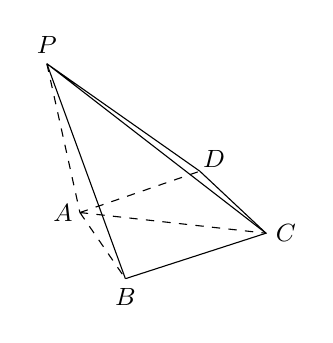
\begin{tikzpicture}[scale=1.05, font=\small]
  \coordinate (P) at (0.75,2.6);
  \coordinate (A) at (1.15,0.8);
  \coordinate (B) at (1.7,0);
  \coordinate (C) at (3.4,0.55);
  \coordinate (D) at (2.6,1.3);
  \draw (P) -- (B)  (P) -- (C)  (P) -- (D);
  \draw (B) -- (C) -- (D);
  \draw[dashed] (P) -- (A);
  \draw[dashed] (A) -- (B)  (A) -- (D)  (A) -- (C);
  \node[above] at (P) {$P$};
  \node[left, inner sep=2.5pt] at (A) {$A$};
  \node[below] at (B) {$B$};
  \node[right] at (C) {$C$};
  \node[above right, inner sep=1pt] at (D) {$D$};
\end{tikzpicture}
\end{center}
\nopagebreak[4]
  (1) 若 $AD\perp PB$，证明：$AD\parallel$ 平面 $PBC$；

  (2) 若 $AD\perp DC$，且二面角 $A\text{-}CP\text{-}D$ 的正弦值为 $\dfrac{\sqrt{42}}{7}$，求 $AD$。

\textbf{解析}

  (1) 若 $AD\perp PB$，证明：$AD\parallel$ 平面 $PBC$；
  (2) 若 $AD\perp DC$，且二面角 $A\text{-}CP\text{-}D$ 的正弦值为 $\dfrac{\sqrt{42}}7$，求 $AD$。

\par\medskip

\textbf{预备：底面的形状（两问共用）}

由 $AB=\sqrt3$，$BC=1$，$AC=2$：
\[AB^{2}+BC^{2}=3+1=4=AC^{2}\]

由勾股定理逆定理，$\angle ABC=90^{\circ}$。

\textbf{建系}：$PA\perp$ 底面，故 $PA$ 与底面内任意直线垂直。取 $A$ 为原点、$AB$ 方向为 $x$ 轴、过 $A$ 且平行于 $BC$ 的方向为 $y$ 轴、$AP$ 为 $z$ 轴：
\[A(0,0,0),\quad B\left(\sqrt3,0,0\right),\quad C\left(\sqrt3,1,0\right),\quad P(0,0,2)\]

（$C$ 的坐标：由 $BC\perp AB$ 且 $BC=1$，从 $B$ 沿 $y$ 轴走 $1$ 个单位。检验 $AC=\sqrt{3+1}=2$ ）

\par\medskip

\textbf{(1) 证明}

设 $D$ 在底面内，$\overrightarrow{AD}=(p,q,0)$。

\[\overrightarrow{PB}=B-P=\left(\sqrt3,\ 0,\ -2\right)\]

由 $AD\perp PB$：
\[\overrightarrow{AD}\cdot\overrightarrow{PB}=\sqrt3\,p+0\times q+0\times(-2)=\sqrt3\,p=0\ \Longrightarrow\ p=0\]

于是 $\overrightarrow{AD}=(0,q,0)$，而
\[\overrightarrow{BC}=C-B=(0,1,0)\]

两者共线，即
\[AD\parallel BC\]

又 $BC\subset$ 平面 $PBC$，且 $AD\not\subset$ 平面 $PBC$（因为 $A$ 不在平面 $PBC$ 内：平面 $PBC$ 的方程可求得为 $2x+\sqrt3z=2\sqrt3$，代入 $A(0,0,0)$ 得 $0\ne2\sqrt3$），

由\textbf{线面平行的判定定理}：
\[AD\parallel\text{\text{平面} }PBC\qquad\blacksquare\]

\par\medskip

\textbf{(2) 解}

设 $D(p,q,0)$，记 $t=|AD|=\sqrt{p^{2}+q^{2}}$。

\textbf{第一步，把条件 $AD\perp DC$ 化成 $p$、$q$ 的关系。}

\[\overrightarrow{DA}=(-p,-q,0),\qquad \overrightarrow{DC}=\left(\sqrt3-p,\ 1-q,\ 0\right)\]

\[\overrightarrow{DA}\cdot\overrightarrow{DC}=-p\left(\sqrt3-p\right)-q(1-q)=p^{2}+q^{2}-\sqrt3p-q=0\]

即得\textbf{关键关系}：
\[\boxed{\sqrt3\,p+q=p^{2}+q^{2}=t^{2}}\qquad(\ast)\]

\textbf{第二步，求两个半平面的法向量。}

\textbf{平面 $ACP$}：含 $A(0,0,0)$、$C\left(\sqrt3,1,0\right)$、$P(0,0,2)$。
\[\boldsymbol n_1=\overrightarrow{AC}\times\overrightarrow{AP}=\left(\sqrt3,1,0\right)\times(0,0,2)\]

\[=\left(1\times2-0\times0,\ 0\times0-\sqrt3\times2,\ 0\right)=\left(2,\ -2\sqrt3,\ 0\right)\]

\[\left|\boldsymbol n_1\right|=\sqrt{4+12}=4\]

\textbf{平面 $DCP$}：含 $D(p,q,0)$、$C\left(\sqrt3,1,0\right)$、$P(0,0,2)$。
\[\overrightarrow{CD}=\left(p-\sqrt3,\ q-1,\ 0\right),\qquad \overrightarrow{CP}=\left(-\sqrt3,\ -1,\ 2\right)\]

\[\boldsymbol n_2=\overrightarrow{CD}\times\overrightarrow{CP}=\left(2(q-1),\ \ 2\sqrt3-2p,\ \ \sqrt3\,q-p\right)\]

\textbf{第三步，代入关系 $(\ast)$ 化简。}

\[\boldsymbol n_1\cdot\boldsymbol n_2=2\cdot2(q-1)+\left(-2\sqrt3\right)\left(2\sqrt3-2p\right)=4q-4-12+4\sqrt3\,p=4\left(\sqrt3\,p+q\right)-16\]

由 $(\ast)$，$\sqrt3p+q=t^{2}$：
\[\boldsymbol n_1\cdot\boldsymbol n_2=4t^{2}-16\]

同样地（把 $\sqrt3p=t^{2}-q$、$p^{2}+q^{2}=t^{2}$ 代入并整理）：
\[\left|\boldsymbol n_2\right|^{2}=-3t^{2}+4q^{2}-2qt^{2}+16\]

\textbf{第四步，用角度条件求解。}

由 $\sin\theta=\dfrac{\sqrt{42}}7$：
\[\cos^{2}\theta=1-\frac{42}{49}=\frac7{49}=\frac17\ \Longrightarrow\ \left|\cos\theta\right|=\frac1{\sqrt7}\]

\[\left|\cos\theta\right|=\frac{\left|\boldsymbol n_1\cdot\boldsymbol n_2\right|}{\left|\boldsymbol n_1\right|\left|\boldsymbol n_2\right|}=\frac{\left|4t^{2}-16\right|}{4\left|\boldsymbol n_2\right|}=\frac1{\sqrt7}\]

\textbf{第五步，联立求 $t$。}

由 $(\ast)$ 与 $p^{2}+q^{2}=t^{2}$ 消去 $p$：把 $p=\dfrac{t^{2}-q}{\sqrt3}$ 代入 $p^{2}+q^{2}=t^{2}$，可解出 $q$ 关于 $t$ 的表达式。

\textbf{试解}（先猜后验，比硬解四次方程快）：取 $t^{2}=3$，则由 $(\ast)$ 有 $\sqrt3p+q=3$ 与 $p^{2}+q^{2}=3$，联立得
\[4p^{2}-6\sqrt3p+6=0\ \Longrightarrow\ 2p^{2}-3\sqrt3p+3=0\ \Longrightarrow\ p=\sqrt3\ \text{\text{或}}\ p=\frac{\sqrt3}2\]

\begin{itemize}
\item $p=\sqrt3\Rightarrow q=0$，即 $D\left(\sqrt3,0,0\right)$——这就是点 $B$，$D$ 与 $B$ 重合，舍去。
\item $p=\dfrac{\sqrt3}2\Rightarrow q=3-\dfrac32=\dfrac32$，即 $D\left(\dfrac{\sqrt3}2,\ \dfrac32,\ 0\right)$ 
\end{itemize}

\textbf{验证这个 $D$}：
\[\overrightarrow{DA}=\left(-\frac{\sqrt3}2,-\frac32,0\right),\quad \overrightarrow{DC}=\left(\frac{\sqrt3}2,-\frac12,0\right),\quad \overrightarrow{DA}\cdot\overrightarrow{DC}=-\frac34+\frac34=0\ \checkmark\]

\[\boldsymbol n_1\cdot\boldsymbol n_2=4\times3-16=-4\]
\[\left|\boldsymbol n_2\right|^{2}=-9+4\times\frac94-2\times\frac32\times3+16=-9+9-9+16=7\]

\[\left|\cos\theta\right|=\frac{|-4|}{4\sqrt7}=\frac1{\sqrt7}\ \checkmark\quad\Longrightarrow\quad\sin\theta=\sqrt{1-\frac17}=\sqrt{\frac67}=\frac{\sqrt{42}}7\ \checkmark\]

完全吻合。

\[AD=t=\sqrt3\]

\textbf{所以 $AD=\sqrt3$。}

\begin{gktip}
\textbf{方法总结}：立体几何中「已知二面角求长度」，把待求长度设为参数 $t$、其余坐标用 $t$ 表示，是通法。本题的加速点在于发现 $(\ast)$ 式使 $\boldsymbol n_1\cdot\boldsymbol n_2$ 直接化为 $4t^2-16$（不含 $p$、$q$），大幅简化了运算。
\end{gktip}

\gkanswer{答案（1）：见解析版}

\gkanswer{答案（2）：$AD=\sqrt3$}

\par\medskip

\end{answer}
\begin{answer}
\gksolhead{18}{17 分}

\textbf{题目}（17 分）：

已知函数 $f(x)=\ln\dfrac{x}{2-x}+ax+b(x-1)^{3}$。

  (1) 若 $b=0$，且 $f'(x)\ge0$，求 $a$ 的最小值；

  (2) 证明：曲线 $y=f(x)$ 是中心对称图形；

  (3) 若 $f(x)>-2$ 当且仅当 $1<x<2$，求 $b$ 的取值范围。

\textbf{解析}

  (1) 若 $b=0$ 且 $f'(x)\ge0$，求 $a$ 的最小值；
  (2) 证明：曲线 $y=f(x)$ 是中心对称图形；
  (3) 若 $f(x)>-2$ 当且仅当 $1<x<2$，求 $b$ 的取值范围。

\par\medskip

\textbf{预备：定义域}

\[\frac x{2-x}>0\ \Longleftrightarrow\ 0<x<2\]

定义域为 $(0,2)$，\textbf{关于 $x=1$ 对称}——这是第 (2) 问的伏笔。

\par\medskip

\textbf{(1) 解}

$b=0$ 时，先把对数拆开：
\[f(x)=\ln x-\ln(2-x)+ax\]

\[f'(x)=\frac1x+\frac1{2-x}+a\]

\textbf{通分化简}（这一步是关键）：
\[\frac1x+\frac1{2-x}=\frac{(2-x)+x}{x(2-x)}=\frac2{x(2-x)}\]

\textbf{求 $\dfrac2{x(2-x)}$ 的最小值}：分母
\[x(2-x)=-x^{2}+2x=1-(x-1)^{2}\]

在 $x\in(0,2)$ 上，$(x-1)^{2}\in[0,1)$，故 $x(2-x)\in(0,1]$，最大值 $1$ 在 $x=1$ 取到。

于是
\[\frac2{x(2-x)}\ge\frac21=2\qquad(x=1\ \text{\text{时取等}})\]

由 $f'(x)\ge0$ 恒成立：
\[\min_{x\in(0,2)}f'(x)=2+a\ge0\ \Longrightarrow\ a\ge-2\]

\textbf{所以 $a$ 的最小值为 $-2$。}

\par\medskip

\textbf{(2) 证明}

\textbf{猜测对称中心}：定义域 $(0,2)$ 的中点是 $x=1$，故猜对称中心为 $\left(1,f(1)\right)$。

先算
\[f(1)=\ln\frac1{2-1}+a\times1+b(1-1)^{3}=\ln1+a+0=a\]

\textbf{验证}：对任意 $t\in(-1,1)$（保证 $1\pm t\in(0,2)$），计算
\[f(1+t)=\ln\frac{1+t}{2-(1+t)}+a(1+t)+bt^{3}=\ln\frac{1+t}{1-t}+a(1+t)+bt^{3}\]
\[f(1-t)=\ln\frac{1-t}{1+t}+a(1-t)+b(-t)^{3}=\ln\frac{1-t}{1+t}+a(1-t)-bt^{3}\]

相加，三部分分别抵消：
\[f(1+t)+f(1-t)=\underbrace{\ln\frac{1+t}{1-t}+\ln\frac{1-t}{1+t}}_{\ln1=0}+\underbrace{a(1+t)+a(1-t)}_{2a}+\underbrace{bt^{3}-bt^{3}}_{0}=2a=2f(1)\]

由中心对称的定义（若对定义域内任意 $t$ 有 $f\left(x_0+t\right)+f\left(x_0-t\right)=2f\left(x_0\right)$，则曲线关于 $\left(x_0,f\left(x_0\right)\right)$ 中心对称），

\textbf{曲线 $y=f(x)$ 关于点 $(1,\ a)$ 中心对称。$\blacksquare$}

\par\medskip

\textbf{(3) 解}

\textbf{第一步，先定出 $a$（这是全题的突破口）。}

条件是\textbf{「当且仅当」}，即
\[f(x)>-2\ \Longleftrightarrow\ x\in(1,2)\]

\begin{itemize}
\item 由于 $x=1$ \textbf{不属于} $(1,2)$，必须有 $f(1)\le-2$，即 $a\le-2$。
\item 若 $a<-2$：由 $f$ 在 $(0,2)$ 上连续且 $f(1)=a<-2$，存在 $\delta>0$ 使得当 $x\in(1,1+\delta)$ 时仍有 $f(x)<-2$。但这些 $x$ 属于 $(1,2)$，按条件应有 $f(x)>-2$，\textbf{矛盾}。
\end{itemize}

故
\[a=-2,\qquad\text{\text{对称中心为} }(1,-2)\]

\textbf{第二步，用对称性把两个条件合并成一个。}

由 (2)，$f(1+t)+f(1-t)=2a=-4$，即
\[f(1-t)=-4-f(1+t)\]

于是
\[f(1+t)>-2\ \Longleftrightarrow\ -4-f(1-t)>-2\ \Longleftrightarrow\ f(1-t)<-2\]

\textbf{这说明}：「$(1,2)$ 上恒 $>-2$」与「$(0,1)$ 上恒 $<-2$」\textbf{自动等价}，只需保证前者。

\textbf{第三步，构造辅助函数并求导。}

令 $t=x-1\in(0,1)$，定义
\[g(t)=f(1+t)+2=\ln\frac{1+t}{1-t}-2(1+t)+bt^{3}+2=\ln\frac{1+t}{1-t}-2t+bt^{3}\]

目标：\textbf{$g(t)>0$ 对一切 $t\in(0,1)$ 成立}。

注意 $g(0)=\ln1-0+0=0$，即 $g$ 从原点出发，所以关键在于 $g$ 的\textbf{初始增长方向}。

求导：
\[\frac{\mathrm d}{\mathrm dt}\ln\frac{1+t}{1-t}=\frac1{1+t}+\frac1{1-t}=\frac2{1-t^{2}}\]

\[g'(t)=\frac2{1-t^{2}}-2+3bt^{2}=2\cdot\frac{1-\left(1-t^{2}\right)}{1-t^{2}}+3bt^{2}=\frac{2t^{2}}{1-t^{2}}+3bt^{2}\]

\textbf{提取公因式 $t^{2}$}（这一步让结构变得清晰）：
\[\boxed{g'(t)=t^{2}\left(\frac2{1-t^{2}}+3b\right)}\]

\textbf{第四步，讨论。}

因 $t^{2}>0$，$g'$ 的符号完全由括号 $h(t)=\dfrac2{1-t^{2}}+3b$ 决定。

注意 $\dfrac2{1-t^{2}}$ 在 $t\in(0,1)$ 上\textbf{单调递增}，其取值范围是 $(2,+\infty)$，\textbf{下确界为 $2$}（在 $t\to0^{+}$ 处趋近但取不到）。

\textbf{情形一：$3b+2\ge0$，即 $b\ge-\dfrac23$。}

此时对一切 $t\in(0,1)$：
\[h(t)=\frac2{1-t^{2}}+3b>2+3b\ge0\]

故 $g'(t)>0$，$g$ 在 $(0,1)$ 上严格递增，从而
\[g(t)>g(0)=0\quad\checkmark\]

条件成立。

\textbf{情形二：$3b+2<0$，即 $b<-\dfrac23$。}

由 $\dfrac2{1-t^{2}}$ 的连续性，存在 $\delta>0$ 使得当 $t\in(0,\delta)$ 时
\[\frac2{1-t^{2}}<-3b\ \Longrightarrow\ h(t)<0\ \Longrightarrow\ g'(t)<0\]

于是 $g$ 在 $(0,\delta)$ 上递减，$g(t)<g(0)=0$，即存在 $x=1+t\in(1,2)$ 使 $f(x)<-2$，\textbf{与条件矛盾}。

\textbf{结论}：
\[b\ge-\frac23,\qquad\text{\text{即}}\qquad b\in\left[-\frac23,\ +\infty\right)\]

\begin{gktip}
\textbf{方法总结}：本题三问层层递进，(2) 的中心对称性是 (3) 的\textbf{关键工具}——它把「双侧条件」压缩成「单侧条件」，工作量减半。第 (3) 问先用「当且仅当」的边界情形锁死 $a=-2$，再把不等式化为 $g(t)>0$、$g(0)=0$ 的标准形式，最后由 $g'$ 在 $t\to0^{+}$ 处的符号定出临界值——这是「恒成立求参数」中最典型的\textbf{端点分析法}。
\end{gktip}

\gkanswer{答案（1）：$a_{\min}=-2$}

\gkanswer{答案（2）：见解析版}

\gkanswer{答案（3）：$b\ge-\dfrac23$}

\par\medskip

\end{answer}
\begin{answer}
\gksolhead{19}{17 分}

\textbf{题目}（17 分）：

设 $m$ 为正整数，数列 $a_1,a_2,\cdots,a_{4m+2}$ 是公差不为 $0$ 的等差数列。若从中删去两项 $a_i$ 和 $a_j\ (i<j)$ 后剩余的 $4m$ 项可被平均分为 $m$ 组，且每组的 $4$ 个数都能构成等差数列，则称数列 $a_1,a_2,\cdots,a_{4m+2}$ 是 $(i,j)$-\textbf{可分数列}。

  (1) 写出所有的 $(i,j)$，$1\le i<j\le6$，使得数列 $a_1,a_2,\cdots,a_6$ 是 $(i,j)$-可分数列；

  (2) 当 $m\ge3$ 时，证明：数列 $a_1,a_2,\cdots,a_{4m+2}$ 是 $(2,13)$-可分数列；

  (3) 从 $1,2,\cdots,4m+2$ 中一次任取两个数 $i$ 和 $j\ (i<j)$，记数列 $a_1,a_2,\cdots,a_{4m+2}$ 是 $(i,j)$-可分数列的概率为 $P_m$，证明：$P_m>\dfrac18$。

\par\medskip

\textbf{解析}

  (1) 写出所有 $(i,j)$，$1\le i<j\le6$，使 $a_1,\cdots,a_6$ 是 $(i,j)$-可分数列；
  (2) 当 $m\ge3$ 时，证明 $a_1,\cdots,a_{4m+2}$ 是 $(2,13)$-可分数列；
  (3) 从 $1,\cdots,4m+2$ 中任取两数 $i<j$，记可分的概率为 $P_m$，证明 $P_m>\dfrac18$。

\par\medskip

\textbf{预备：把问题「翻译」成整数问题（做本题的第一步）}

设等差数列首项 $a_1$、公差 $d\ne0$，则 $a_k=a_1+(k-1)d$。

若干项 $a_{k_1},a_{k_2},a_{k_3},a_{k_4}$ 构成等差数列
\[\iff a_{k_2}-a_{k_1}=a_{k_3}-a_{k_2}=a_{k_4}-a_{k_3}\iff \left(k_2-k_1\right)d=\left(k_3-k_2\right)d=\left(k_4-k_3\right)d\]

因 $d\ne0$ 可约去，条件\textbf{只与下标有关}：
\[k_2-k_1=k_3-k_2=k_4-k_3\]

\textbf{结论}：可以直接把 $a_k$ 看成整数 $k$，问题变为——

\begin{gktip}
从 $\{1,2,\cdots,4m+2\}$ 中删去 $i$、$j$ 后，能否把剩下的 $4m$ 个整数分成 $m$ 组，每组 $4$ 个数成等差数列？
\end{gktip}

\par\medskip

\textbf{(1) 解}

此时 $m=1$，$4m+2=6$。删去两个数后剩 $4$ 个数，须\textbf{自身构成一个等差数列}。

\textbf{穷举 $\{1,\cdots,6\}$ 中的四项等差子列}：设公差为 $e\ge1$，四项跨度为 $3e$，需 $3e\le6-1=5$，故 $e=1$。

公差为 $1$ 的四项等差数列（即四个连续整数）：
\[\{1,2,3,4\},\qquad\{2,3,4,5\},\qquad\{3,4,5,6\}\]

对应删去的两项分别为：
\[\{5,6\}\ \to\ (i,j)=(5,6);\qquad \{1,6\}\ \to\ (1,6);\qquad \{1,2\}\ \to\ (1,2)\]

\textbf{所以 $(i,j)=(1,2)$、$(1,6)$、$(5,6)$。}

\par\medskip

\textbf{(2) 证明}

删去 $2$ 和 $13$ 后，剩余的数为
\[\{1\}\ \cup\ \{3,4,5,\cdots,12\}\ \cup\ \{14,15,\cdots,4m+2\}\]

\textbf{计数校验}：$1+10+\left(4m+2-14+1\right)=1+10+(4m-11)=4m$ 

\textbf{构造分组}：

\textbf{前三组}取公差为 $3$ 的四元组：
\[\{1,\ 4,\ 7,\ 10\},\qquad\{3,\ 6,\ 9,\ 12\},\qquad\{5,\ 8,\ 11,\ 14\}\]

三组共用去 $12$ 个数，把它们排序即
\[1,3,4,5,6,7,8,9,10,11,12,14\]

\textbf{恰好就是} $\{1\}\cup\{3,\cdots,12\}\cup\{14\}$ 的全部元素——不重不漏 

\textbf{其余各组}：剩下的是
\[\{15,\ 16,\ \cdots,\ 4m+2\}\]

这是 $4m+2-15+1=4m-12=4(m-3)$ 个\textbf{连续整数}，按每 $4$ 个连续一组：
\[\{15,16,17,18\},\ \{19,20,21,22\},\ \cdots\]

共 $m-3$ 组，每组公差为 $1$，均为等差数列 

（$m\ge3$ 保证 $m-3\ge0$；当 $m=3$ 时该部分为空集，前三组已用完全部数。）

\textbf{总组数}：$3+(m-3)=m$ 

\textbf{所以当 $m\ge3$ 时，数列是 $(2,13)$-可分数列。$\blacksquare$}

\par\medskip

\textbf{(3) 证明}

\textbf{思路}：不必刻画出\textbf{所有}可分的 $(i,j)$（那非常复杂），只需构造出\textbf{足够多}的可分对，使其占比已超过 $\dfrac18$ 即可。

\textbf{总的取法数}：
\[N=\binom{4m+2}2=\frac{(4m+2)(4m+1)}2=(2m+1)(4m+1)\]

\par\medskip

\textbf{第一族可分对：$i\equiv1\pmod 4$ 且 $j\equiv2\pmod 4$}

设 $i=4s+1$、$j=4t+2$。删去它们后，剩余的数被自然分成三段：

\begin{center}
\begin{tabular}{llc}
\toprule
段 & 元素 & 个数 \\
\midrule
前段 & $1,\cdots,i-1$ & $i-1=4s$ \\
中段 & $i+1,\cdots,j-1$ & $j-i-1=4(t-s)$ \\
后段 & $j+1,\cdots,4m+2$ & $4m+2-j=4(m-t)$ \\
\bottomrule
\end{tabular}
\end{center}

\textbf{三段的长度都是 $4$ 的倍数}，因此每段各自按「连续四个一组」分组即可，全部组都是公差为 $1$ 的等差数列 

\textbf{计数}：$i<j\iff 4s+1<4t+2\iff 4s<4t+1\iff s\le t$。
其中 $s,t\in\{0,1,\cdots,m\}$（因 $i\le4m+1$、$j\le4m+2$）。

满足 $0\le s\le t\le m$ 的数对个数为
\[\binom{m+1}2+(m+1)=\frac{(m+1)(m+2)}2\]

\par\medskip

\textbf{第二族可分对：$i\equiv2\pmod4$、$j\equiv1\pmod4$，且 $j-i\ge7$}

设 $i=4s+2$、$j=4t+1$，条件 $j-i\ge7$ 等价于 $t\ge s+2$。

删去后，把剩余数拆成三部分：

\[\underbrace{\{1,\cdots,4s\}}_{4s\ \text{\text{个，连续分组}}}\ \cup\ \underbrace{\{4s+1\}\cup\{4s+3,\cdots,4t\}\cup\{4t+2\}}_{\text{\text{中间部分}}}\ \cup\ \underbrace{\{4t+3,\cdots,4m+2\}}_{4(m-t)\ \text{\text{个，连续分组}}}\]

\textbf{中间部分的元素个数}：
\[1+\left(4t-4s-2\right)+1=4(t-s)\]

是 $4$ 的倍数  记 $k=t-s\ge2$，把中间部分统一减去 $4s$，即需要对集合
\[S_k=\{1\}\cup\{3,4,\cdots,4k\}\cup\{4k+2\}\qquad\left(\left|S_k\right|=4k\right)\]
分组。

\textbf{分组构造（按 $k$ 的奇偶）}：

\begin{itemize}
\item \textbf{$k$ 为偶数}：把 $S_k$ 按奇偶拆开——
\end{itemize}
  奇数部分 $1,3,5,\cdots,4k-1$ 共 $2k$ 个，偶数部分 $4,6,\cdots,4k,4k+2$ 共 $2k$ 个。
  因 $k$ 为偶数，$2k$ 是 $4$ 的倍数，两部分各自按「相邻四个」分组，每组公差为 $2$ 
  （例：$k=2$ 时 $S_2=\{1,3,4,5,6,7,8,10\}$，分为 $\{1,3,5,7\}$ 与 $\{4,6,8,10\}$。）

\begin{itemize}
\item \textbf{$k$ 为奇数}（$k\ge3$）：先取三组公差为 $3$ 的四元组
\end{itemize}
\[\{1,4,7,10\},\quad\{3,6,9,12\},\quad\{5,8,11,14\}\]
  它们恰好用完 $\{1,3,4,\cdots,12,14\}$；剩余为
\[\{13,15,17,\cdots,4k-1\}\cup\{16,18,\cdots,4k+2\}\]
  两个等差子集各含 $2(k-3)$ 个元素，因 $k$ 为奇数故 $k-3$ 为偶数、$2(k-3)$ 是 $4$ 的倍数，各自按相邻四个分组即可 
  （例：$k=3$ 时剩余为空；$k=5$ 时剩余分为 $\{13,15,17,19\}$ 与 $\{16,18,20,22\}$。）

\textbf{计数}：$s\ge0$、$t\le m$、$t\ge s+2$，故
\[\#\{(s,t)\}=\sum_{s=0}^{m-2}\left(m-s-1\right)=\sum_{r=1}^{m-1}r=\frac{m(m-1)}2\]

\par\medskip

\textbf{第三步，合并计数并放缩}

两族的 $(i,j)$ 互不重复（第一族 $i\equiv1$、第二族 $i\equiv2\pmod4$），故可分对数
\[M\ \ge\ \frac{(m+1)(m+2)}2+\frac{m(m-1)}2\]

\[=\frac{m^{2}+3m+2+m^{2}-m}2=\frac{2m^{2}+2m+2}2=m^{2}+m+1\]

于是
\[P_m=\frac{M}{N}\ \ge\ \frac{m^{2}+m+1}{(2m+1)(4m+1)}=\frac{m^{2}+m+1}{8m^{2}+6m+1}\]

\textbf{最后一步，验证它确实大于 $\dfrac18$：}
\[8\left(m^{2}+m+1\right)-\left(8m^{2}+6m+1\right)=8m^{2}+8m+8-8m^{2}-6m-1=2m+7>0\]

即
\[\frac{m^{2}+m+1}{8m^{2}+6m+1}>\frac18\]

\textbf{所以}
\[P_m>\frac18\qquad\blacksquare\]

\begin{gktip}
\textbf{方法总结}：这是近年新高考卷中难度最高的压轴题之一，但它的破题逻辑是清晰的三步：
1. \textbf{翻译}——等差子列只与\textbf{下标}有关，把抽象数列问题降为整数分组问题（这一步不做，后面寸步难行）；
2. \textbf{构造}——(2) 给出了一个"样板构造"：\textbf{用公差为 3 的组去消化边界上的零散数，用连续四个一组去消化整齐的长段}。(3) 正是把这个样板推广成两个可分对家族；
3. \textbf{放缩}——(3) 不要求刻画全部可分对，只要构造出的两族已经占到 $\dfrac18$ 以上即可。\textbf{能想到"只证下界、不求精确值"，是本题最重要的解题意识。}

从考试策略看：(1) 是送分的（3 分），(2) 只需给出一个构造（可拿 6 分），(3) 是真正的区分点。及格线到 120 分段的学生应当\textbf{主攻 (1)(2)，果断放弃 (3)}。
\end{gktip}

\gkanswer{答案（1）：$(1,2)$、$(1,6)$、$(5,6)$}

\gkanswer{答案（2）：见解析版}

\gkanswer{答案（3）：见解析版}

\end{answer}